\section{Experiments}

\begin{figure}[!tb]
%\begin{figure}[t]
  \centering
  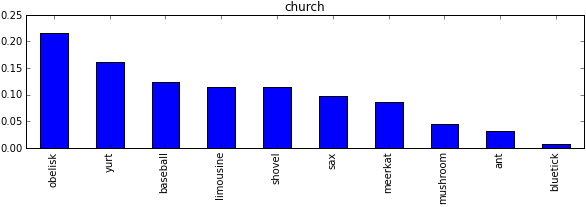
\includegraphics[width=0.5\textwidth]{figs/word2vec_church.png}
  \caption{
    The Word2Vec similarity scores for \emph{church}. Other structures, such as
    \emph{obelisk} and \emph{yurt} (a type of tent) were the closest in
    similarity. \emph{Bluetick} (a type of dog) was the most distant.
  }
  \label{fig:word2vec_similarities}
\end{figure}

% \begin{table}[!tb]
%   \centering
%   \begin{tabular}{|c|c|c|}
%     \hline
%       & \textbf{1-Hot Labels} & \textbf{Word2Vec Labels} \\
%     \hline
%       \textbf{VGG-16} & 0.2167 & 0.2091 \\
%     \hline
%       \textbf{4-layer CNN} & 0.1091 & 0.1864 \\
%     \hline
%   \end{tabular}
%   \caption{
%     The training results after 50 epochs of using 1-hot labels vs. using soft
%     labels from Word2Vec.
%   }
%   \label{tbl:results}
% \end{table}

% We will evaluate and compare the performance of deep convolutional neural
% networks trained on ImageNet with soft labels and 1-hot labels.
% We will train the VGG-16 model \cite{simonyan2014very} from scratch, and see
% how well it learns using the different labeling schemas. Our goal is to try to
% find the optimal hyperparameters for which soft label training will outperform
% 1-hot labels.
% We will also analyze the errors made by both models to see how semantically
% relevant the models are.
% We plan to use the evaluation method introduced in \cite{zhao2011large} for
% testing semantically relevant errors.

% We will also experiment with pretrained networks and different architectures to
% see how effectively they can learn with soft labels compared to 1-hot labels.
% In \cite{hinton2015distilling} the authors showed that they can use soft labels
% to train simpler models quickly that perform nearly as well as the advanced
% models with many more parameters. We hope to mirror these results, but using
% semantic weights for the learning targets.
% Finally, we plan to experiment with training on fewer examples to see if our
% approach can help in cases where labeled data is limited.

% Throughout all of our experiments, we will compare different schemes for
% obtaining the soft labels. We will use Word2Vec, WordNet, and possibly visual
% similarity, and discover optimal distributions for these weights.
% We hope to look at different linguistic semantic similarity measures and
% compare them with visual similarity measures, and analyze which object
% categories relate well in both the visual and semantic domain.

We consider two class sets, each of which were taken from ImageNet. The first
class set consists of the following five classes:
\emph{sax},
\emph{church},
\emph{obelisk},
\emph{yurt}, and
\emph{limousine}.
We refer to this class set as C5.
The next class set consists of the following ten classes:
\emph{sax},
\emph{limousine},
\emph{shovel},
\emph{baseball},
\emph{meerkat},
\emph{church},
\emph{yurt},
\emph{obelisk},
\emph{bluetick}, and
\emph{mushroom}.
We refer to this class set as C10 throughout.
The next class set consists of the following ten classes:
\emph{limousine},
\emph{fiddler crab},
\emph{baseball},
\emph{dalmatian},
\emph{barber chair},
\emph{church},
\emph{lakeside},
\emph{mushroom},
\emph{measuring cup}, and
\emph{projectile}.

\begin{figure*}[t]
%\begin{figure}[t]
  \centering
  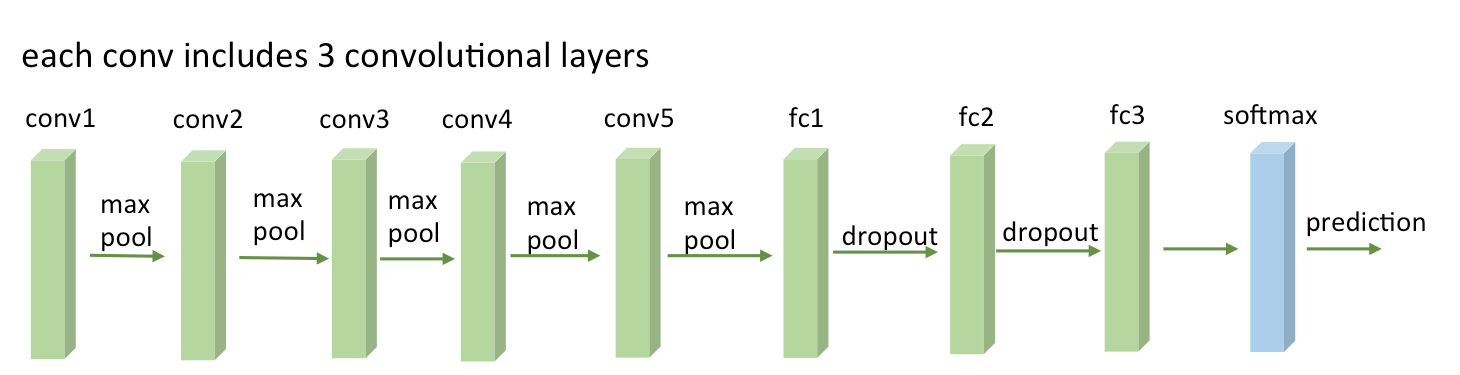
\includegraphics[width=1.0\textwidth]{figs/vgg16arch.png}
  \caption{
      VGGNet architecture. Image credit
      http://blog.christianperone.com/tag/keras/.
  }
  \label{fig:vgg16arch}
\end{figure*}

For each class set, we train a VGGNet with various soft labeling schemes. The
VGGNet architecture is pictured in Figure \ref{fig:vgg16arch}. The only
modification to the architecture we made was to vary the number of
predicted class probabilities based on the class set.

Figures \ref{fig:5_1-train_100} and \ref{fig:5_1-train_1260} shows results on
the C5 class set. We see that the soft-labeling scheme consistently outperform
the one-hot labeling scheme and the random labeling scheme for the case of 100
training examples per class. However, the performance is less significant when
the number of training examples increases to 1260. This can be explained by the
fact that soft labeling schemes become less valuable when the number of training
examples increases. Soft labeling schemes to be particularily useful when the
number of training examples are small.

\begin{figure}[!tb]
%\begin{figure}[t]
  \centering
  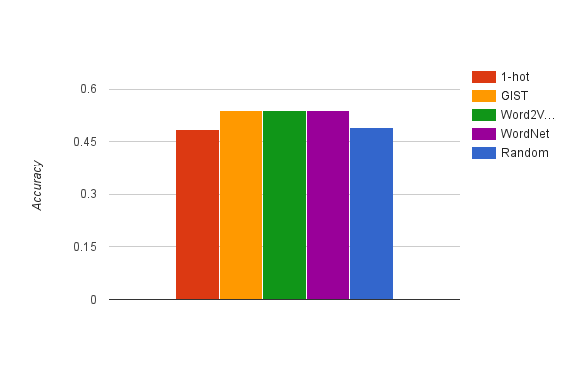
\includegraphics[width=0.5\textwidth]{figs/5_1-train_100.png}
  \caption{
      Accuracies for a variety of label sharing schemes on C5 class set. Our
      soft-labeling schemes consistently outperform one hot and random labeling
      schemes, especially with a small number of training examples.
  }
  \label{fig:5_1-train_100}
\end{figure}

\begin{figure}[!tb]
%\begin{figure}[t]
  \centering
  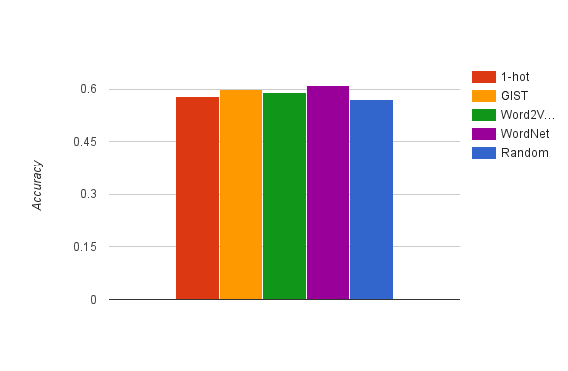
\includegraphics[width=0.5\textwidth]{figs/5_1-train_1260.png}
  \caption{
      Accuracies for a variety of label sharing schemes on C5 class set. With
      more training examples, performance gains become less significant for
      soft-labeling schemes.
  }
  \label{fig:5_1-train_1260}
\end{figure}

Figures \ref{fig:10_1-train_100} and \ref{fig:10_1-train_1260} demonstrate the
performance of various labeling schemes on the C10 dataset. Once again we see
improved performance for the soft labeling schemes over one-hot and random soft
labeling schemes. The performance boost seems to be a bit more significant here
than in the five-class case, perhaps owing to the fact that the increase in the
number of classes provides more of an opportunity to convey more relationships
between classes.

\begin{figure}[!tb]
%\begin{figure}[t]
  \centering
  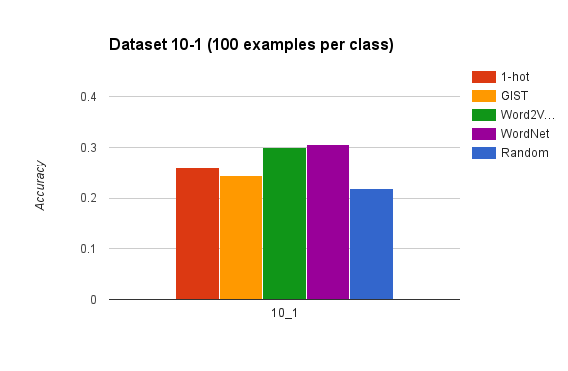
\includegraphics[width=0.5\textwidth]{figs/10_1-train_100.png}
  \caption{
      Accuracies for a variety of label sharing schemes on C10 class set. Our
      soft-labeling consistently outperform one-hot labeling and random
      labeling.
  }
  \label{fig:10_1-train_100}
\end{figure}

\begin{figure}[!tb]
%\begin{figure}[t]
  \centering
  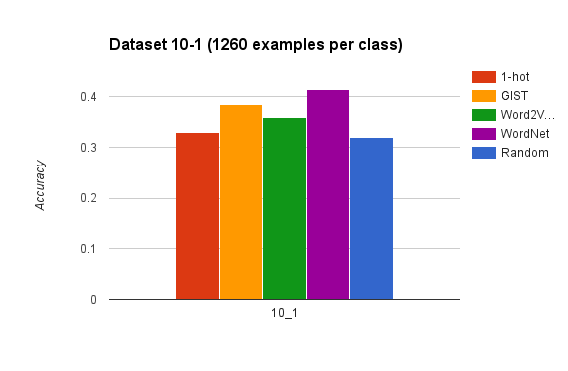
\includegraphics[width=0.5\textwidth]{figs/10_1-train_1260.png}
  \caption{
      Accuracies for a variety of label sharing schemes on C10 class set. Our
      soft-labeling consistently outperform one-hot labeling and random
      labeling.
  }
  \label{fig:10_1-train_1260}
\end{figure}

The fact that GIST soft-labels performed well was a nice surprise for us. Even
though visual similarity between classes is often noisy, it still provides
enough of a valuable signal to improve learning (most of the time).

% As a proof of concept, we trained two models on a small amount of data from
% ImageNet. We used 11 ImageNet classes -
% \emph{
%   saxophone,
%   limousine,
%   shovel,
%   baseball,
%   meerkat,
%   church,
%   yurt,
%   obelisk,
%   bluetick,
%   mushroom,
%   ant
% } -
% each with 100 training examples and 20 test examples.
% Using Word2Vec trained on articles from Google News, we extracted similarity
% scores between these categories. The similarity scores for \emph{church} are
% shown in Figure \ref{fig:word2vec_similarities}.

% We trained the VGG-16 model as well as a simpler four-layer CNN on this data
% set. Our average results over three experimental trials can be seen in Table
% \ref{tbl:results}.
% While the results for the VGG-16 model are similar in both cases, there is a
% clear boost in performance on the simpler model. Our naivly-selected soft
% labels perform almost as well as VGG-16 despite being a significantly inferior
% architecture.
% The overall poor performance can be attributed to the tiny training data set.

% Naturally, we will run experiments with much larger training sets and we will
% search for the best hyperparameters.
% We will also work on improving the design of the soft labels, which were not
% adjusted at all for this experiment - we just took the cosine similarity
% between the raw Word2Vec features.


\begin{figure}[!tb]
%\begin{figure}[t]
  \centering
  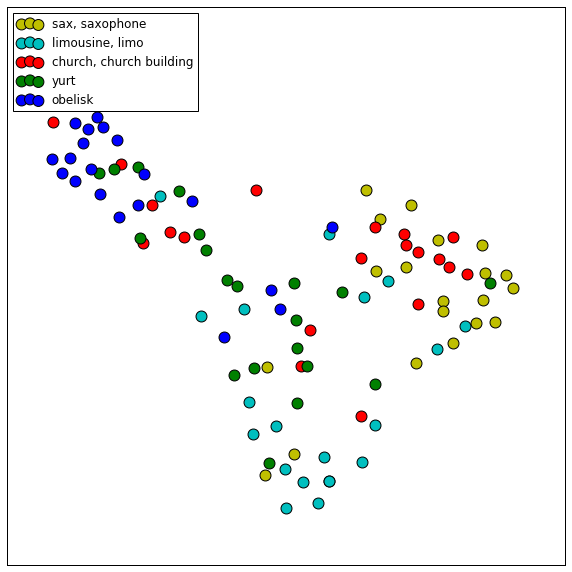
\includegraphics[width=0.5\textwidth]{figs/tsne.png}
  \caption{
      t-SNE visualization of predicted softmax probabilities for C5 test set.
      Notice \emph{yurt} and \emph{obelisk,} two labels with a high semantic
      score, cluster together.
  }
  \label{fig:tsne}
\end{figure}

\begin{table}[!tb]
    \centering
    \begin{tabular}{lrr}
         & WN-PATH & WN-ZHAO\\
        \hline
        WordNet + GIST & 0.261114 & 0.456478\\
        word2vec & 0.2995 & 0.550523\\
        WordNet & 0.36027 & \textbf{0.581415}\\
        Dependency & 0.091352 & 0.394429\\
        One Hot & \textbf{0.361664} & 0.533101\\
    \end{tabular}
  \label{tbl:semantic_misses}
  \caption{
      Semantic evaluation on only missed examples. Models trained
      with soft labels generally make more semantically meaningful errors. Our
      semantic evaluation criterias are similar to \cite{zhao2011large}, with a
      slight variation.
  }
\end{table}

Table \ref{tbl:semantic_misses} attempts to get a handle on the types of errors
that each model is making. We use a similar semantic evaluation metric to
\cite{zhao2011large}, but with the following deviation: each of the evaluation
metrics is defined by an affinity matrix. If the correct prediction is made, the
model gets 1 point. If a model predict class $j$, but the correct class was $i$,
then the model gets a point value equal to $A_{ij}$.

We can see that the model trained on one hot labels performs highest on WN-PATH,
but both word2vec and WordNet perform higher on WN-ZHAO. WN-ZHAO is based on the
affinity matrix calculated with equation \ref{eq:wordnet_dist}. We believe that
performance is higher on WN-ZHAO for both the WordNet and word2vec soft labels
because of the due to the diffuse property of the WN-PATH affinity matrix versus
the sparseness of the WN-ZHAO affinity matrix. Because WN-PATH is more diffuse,
the one-hot model does not get penalized as harshly for making a bad semantic
mistake, whereas it gets penalized much more harshly with WN-ZHAO. The score is
slightly inflated for the WordNet model because the WordNet model was trained
directly using the affinity matrix, but the word2vec results require no such
disclaimer.

Figure \ref{fig:tsne} shows a t-SNE plot of the predicted softmax probability
vectors for the C5 class set with word2vec soft labels. We notice that images of
yurts and obelisks are clustered close together, indicating that in images of
both, both of them often received high probability values. t-SNE plots are
usually performed on the final hidden layer of a CNN, but performing t-SNE on
the softmax probabilities highlights the goal of our approach.

% \begin{table*}[t]
%     \centering
%     \begin{tabular}{lrrrrr}
%          & WN-PATH & WN-WUP & WN-ZHAO & GIST & 1-HOT\\
%         \hline
%         WordNet + GIST & 0.603798 & 0.729889 & 0.716476 & 0.703609 & 0.57\\
%         WordNet & 0.585442 & 0.725779 & 0.710825 & 0.678581 & 0.55\\
%         word2vec & 0.624362 & 0.755722 & 0.742397 & 0.708035 & 0.59\\
%         Dependency Embeddings & 0.535218 & 0.71633 & 0.696365 & 0.652365 &
%         0.49\\
%         One Hot & 0.622404 & 0.74834 & 0.735746 & 0.711471 & 0.59\\
%     \end{tabular}
%     \caption{
%         Semantic evaluation numbers for different soft labeling schemes. The
%         word2vec labeling scheme achieves the same raw accuracy as one hot, but
%         scores higher on WordNet metrics.
%     }
%   \label{tbl:semantic_eval}
% \end{table*}


%\subsection{CNN Architecture}
%
%TODO.
